
\فصل{مفاهیم اولیه}

% stroke types
% aspects
% thrombectomy
% aspect slices
% ct and dicom

% segmentation
% augmentation
% transfer learning
% pretrained models
% cross validation

در این فصل به ذکر برخی مفاهیم اولیه‌ی مورد ارجاع در ادامه‌ی پایان‌نامه پرداخته می‌شود.
این مفاهیم در دو دسته‌ی پزشکی و فنی قابل بررسی هستند.
در ابتدا، مبانی پزشکی موضوع پروژه و نکاتی حول تصاویر پزشکی مورد استفاده به اختصار شرح داده می‌شود.
در ادامه نیز نکاتی در رابطه با هسته‌ی فنی پروژه و روش‌های مورد استفاده در یادگیری ماشین ذکر می‌گردد.
به این ترتیب، این فصل می‌تواند در دست‌یابی به یک دانش مشترک در میان متخصصان هر دو حوزه اثربخش باشد.

\قسمت{مفاهیم پزشکی}

\زیرقسمت{سکته‌ی مغزی}

انواع سکته‌های مغزی شامل دو دسته‌ی کلی سکته‌های انسدادی
\footnote{ischemic}
و خونریزی
\footnote{haemorrhagic} 
هستند.
سکته‌ی مغزی انسدادی به علت قطع شدن جریان خون به بخشی از مغز رخ می‌دهد که باعث از دست رفتن ناگهانی عملکرد آن ناحیه می‌شود.
در مقابل، سکته‌ی مغزی خونریزی از پاره‌شدن یک رگ خونی و یا ساختار غیر طبیعی عروقی نشأت می‌گیرد.
در یک نگاه کلی، تقریبا ۸۰٪ بیماران سکته‌ی مغزی، در دسته‌ی اول، یعنی سکته‌ی انسدادی، قرار می‌گیرند.
%https://www.ncbi.nlm.nih.gov/pmc/articles/PMC6288566/ Stroke in the 21st Century: A Snapshot of the Burden, Epidemiology, and Quality of Life
این دو نوع سکته‌ی مغزی، ظاهر متفاوتی در تصاویر CT به خود می‌گیرند.
تصویر ~\ref{fig:ischemic-harmorhagic} این تفاوت را نشان می‌دهد.
همانطور که در این تصویر نمایان است، عموما تشخیص ناحیه‌ی درگیری
در سکته‌ی خونریزی ساده‌تر است و در مقابل، تشخیص این نواحی در سکته‌ی انسدادی، ظرافت و دقت بیشتری نیاز دارد.
همانطور که در تعریف امتیاز ASPECT خواهد آمد، عنوان پژوهش حاضر نیز، زیرمجموعه‌ی 
سکته‌های انسدادی قرار می‌گیرد و تمام مفاهیم مورد اشاره در این پایان‌نامه و تمام تصاویر مورد استفاده نیز به این نوع سکته اشاره خواهند داشت.

\begin{figure}[ht]
\centering
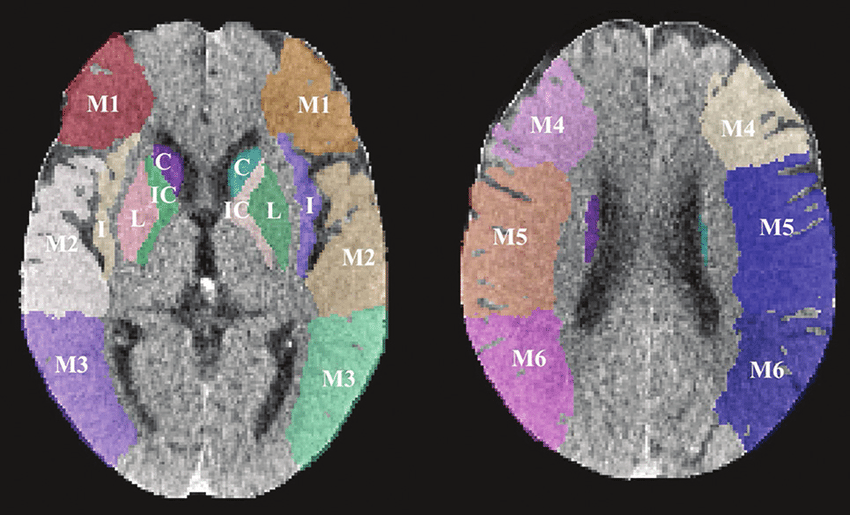
\includegraphics[width=\textwidth, keepaspectratio]{aspects-regions.png}
\caption[]{انواع سکته‌ی مغزی در تصاویر ،CT برش مغزی A یک نمونه سکته‌ی انسدادی و برش B یک نمونه از سکته‌ی خونریزی در این تصاویر را نشان می‌دهد.}
\label{fig:ischemic-haemorrhagic}
\end{figure}
%Ischemic and hemorrhagic brain injury during venoarterial-extracorporeal membrane oxygenation
        
\زیرقسمت{امتیاز ASPECT}

ASPECTS 
\footnote{The Alberta Stroke Program Early CT Score}
یک امتیاز عددی از ۱ تا ۱۰ است که میزان پیشرفت تغییرات حاصل از سکته‌ی انسدادی را 
نشان می‌دهد.
 امتیاز‌دهی ،ASPECT 
 محدوده‌ی رگ مغزی میانی را به ۱۰ ناحیه‌ی مشخص تقسیم می‌کند (تصویر ~\ref{fig:aspects-regions}).
 امتیازدهی  از ۱۰ آغاز می‌شود و به ازای هر کدام از این ۱۰ ناحیه که علائم کاهش جریان 
 خون را نشان می‌دهند، یک امتیاز از ۱۰ کم می‌شود.
 این امتیاز برای تجویز لخته‌زدایی‌های درون‌رگی و برون‌رگی برای بیماران به‌کار می‌آید.
 %ASPECTS (Alberta Stroke Program Early CT Score) Measurement Using Hounsfield Unit Values When Selecting Patients for Stroke Thrombectomy

\begin{figure}[ht]
\centering
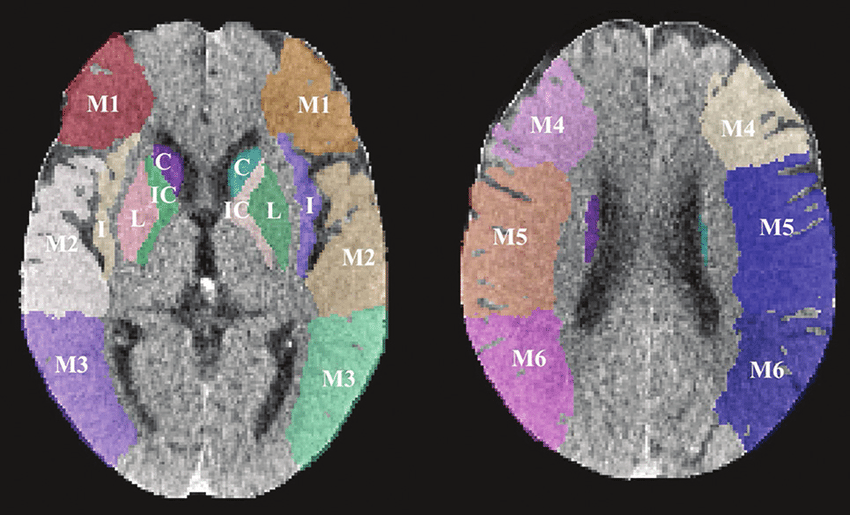
\includegraphics[width=\textwidth, keepaspectratio]{aspects-regions.png}
\caption[]{نواحی ASPECTS در دو برش از مغز. ۱۰ ناحیه شامل ،I ،C ،L ،IC \lr{M6}-\lr{M1}.}
\label{fig:aspects-regions}
\end{figure}
%Kuang, Hulin & Najm, Mohamed & Chakraborty, Debabrata & Maraj, Nicholas & Sohn, Sung-Il & Goyal, Mayank & Hill, Michael & Demchuk, Andrew & Menon, Bijoy & Qiu, Wu. (2018). Automated ASPECTS on Non-Contrast CT Scans in Acute Ischemic Stroke Patients Using Machine Learning. American Journal of Neuroradiology. 10.3174/ajnr.A5889. 

این امتیاز 
به این منظور طراحی شده‌است که 
در تشخیص بیمارانی که نتایج بهتری از لخته‌زدایی درون‌رگی
کسب خواهند کرد،‌کمک کننده باشد.
بعد‌ها از این امتیاز برای تشخیص بیمارانی استفاده شد که برای اعمال لخته‌زدایی برون‌رگی مناسب نیستند.
درواقع عملیات باز کردن رگ‌ها 
\footnote{recanalization}
در بیمارانی که علائم سکته‌ی انسدادی در نواحی وسیعی از مغزشان گسترده شده، می‌تواند بی‌اثر یا حتی زیان‌بار باشد.
اخیراً هم این امتیاز در
مجموعه‌ی دستور‌العمل‌های مدیریت سکته‌ی مغزی
انجمن قلب آمریکا به عنوان 
 یک معیار کلیدی در تجویز 
 لخته‌زدایی برون‌رگی عنوان شده‌است.
 به نحوی که این روش درمانی برای بیمارانی با امتیاز $ASPECTS\geq 6$، توصیه می‌شود.
%ASPECTS (Alberta Stroke Program Early CT Score) Measurement Using Hounsfield Unit Values When Selecting Patients for Stroke Thrombectomy
با این تفسیر، مشخص می‌شود علی‌رغم ۱۰ امتیازی بودن ASPECTS، معمولا آن‌چه که اهمیت دارد، تنها یک حد آستانه بر روی این امتیاز است.
به این نوع از امتیازدهی که وضعیت بیماران را به دو دسته‌ی بالا و پایین یک آستانه (مثلا $ASPECTS\geq6$) تقسیم می‌کند، امتیاز دوبخشی‌شده‌ی
\footnote{dichotomized}
ASPECTS می‌گویند.
لازم به ذکر است که خروجی نهایی پژوهش حاصل و نتایج گزارش‌شده برای آن نیز، از نوع امتیازدهی دو‌بخشی خواهند بود.

\زیرقسمت{نحوه‌ی امتیاز‌دهی ASPECT از روی تصاویر مغزی}

همانطور که پیش‌تر ذکر شد، امتیاز ASPECTS برای یک فرد سالم برابر با ۱۰ می‌باشد و به ازای هر یک از ۱۰ ناحیه‌ی تعیین‌شده‌ای که در اثر انسداد عروقی، آسیب دیده‌باشد، یک واحد از این امتیاز کسر می‌شود تا در حادترین وضعیت به صفر برسد.
دقت داریم که هر کدام از نواحی، به صورت قرینه در دو نیم‌کره‌ی مغز وجود دارند و در هر سمتی از مغز که آسیب دیده باشند، مجموعا تنها یک امتیاز از این ۱۰ امتیاز کم می‌کنند.
\footnote{البته در اکثر نمونه‌های سکته‌ی مغزی انسدادی، آسیب‌دیدگی تنها در یک نیم‌کره گسترش می‌یابد.}
هر یک از ۱۰ ناحیه‌ی ASPECTS فوق‌الذکر، درواقع یک حجم و ناحیه‌ی سه‌بعدی در مغز را شامل می‌شوند.
تصویر ~\ref{fig:aspects-regions} نیز شمایی از این نواحی را تنها در برش‌های خاصی از مغز نمایش داده‌است.
در حالی که هر کدام از این نواحی، در چندین برش از مغز گسترده شده‌اند.
از جنبه‌ی نظری، درست آن است که در تشخیص امتیاز ASPECTS، تمام حجم مربوط به یک ناحیه در نظر گرفته شود.
اما در عمل، معمولا تنها چند برش از مغز به منظور تشخیص، مورد بررسی قرار می‌گیرند.\\

گستردگی نواحی ده‌گانه‌ی ASPECTS در ۸ برش مغزی در تصویر ~\ref{fig:aspects-slices} قابل مشاهده است.
اگرچه پژوهش‌هایی وجود دارند که امتیاز ASPECT را از روی تصاویر سه‌بعدی محاسبه می‌کنند اما 
ساختارشناسی نواحی ASPECTS تشخیص انسانی آن عموما بر روی همین تعداد محدود برش انجام می‌شود.
در بخش کارهای پیشین خواهد آمد که پژوهش‌هایی که ASPECTS را به صورت سه‌بعدی محاسبه نمی‌کنند، غالبا تنها دو برش از مغز را ارزیابی می‌کنند.
این در حالی است که روش پیشنهادی این پژوهش، انطباق بیشتری با روش انسانی مورد استفاده در مراکز درمانی دارد و 
آسیب‌دیدگی نواحی ده‌گانه را در حجم وسیع‌تری از مغز مورد بررسی قرار می‌دهد. جزئیات این مسئله در بخش روش پیشنهادی خواهد آمد.

\begin{figure}[ht]
\centering
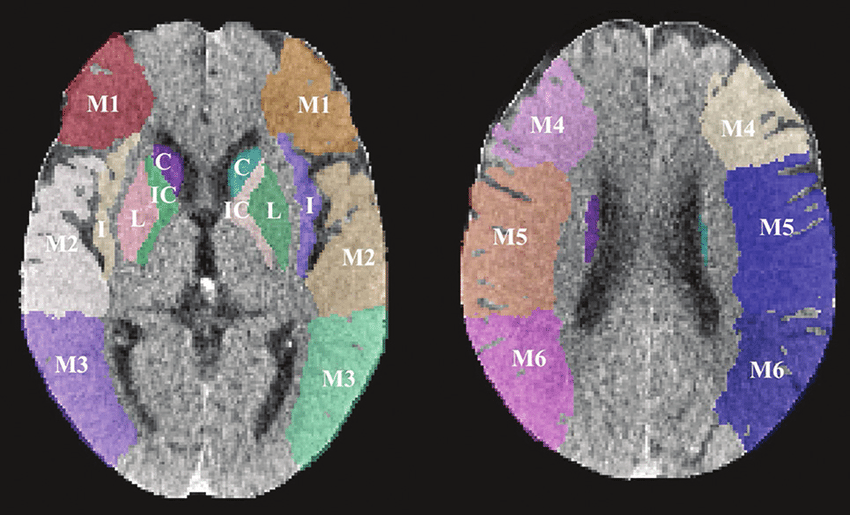
\includegraphics[width=\textwidth, keepaspectratio]{aspects-regions.png}
\caption[]{گستردگی نواحی ده‌گانه‌ی ASPECTS در برش‌های مغز.}
\label{fig:aspects-slices}
\end{figure}
%Minds treating brains: understanding the interpretation of non-contrast CT ASPECTS in acute ischemic stroke

